\documentclass{beamer}
\usepackage{../../../resources/themes/algolymp-light}
\usepackage{booktabs}
\usepackage{amssymb}
\usepackage{tikz}

\title{Metoda Greedy}
\subtitle{Problema spectacolelor $\cdot$ Diverse probleme}
\author{Andrei Mihai Ciobanu}
\institute{Algolymp Summer School}
\date{}
\titlegraphic{
\includegraphics[width=3cm]{../../../resources/algolymp-logo.png}}
\setbeamertemplate{frame footer}{Algolymp Summer School}

% ============================================================
\begin{document}

\begin{frame}
  \titlepage
\end{frame}

\begin{frame}{Cuprins}
  \tableofcontents[hideallsubsections]
\end{frame}

% ============================================================
\section{Ce este Greedy?}

\begin{frame}{Motivație \textemdash{} Problema restului}
  \begin{block}{Problemă}
    Se dau monede de valori $1$, $5$, $10$, $50$ lei.
    Trebuie dat rest de $R$ lei folosind \textbf{cât mai puține monede}.
  \end{block}
  \smallskip
  \textbf{Strategie naturală:} la fiecare pas, se alege
  \textbf{cea mai mare monedă} care nu depășește restul rămas.
  \smallskip
  \begin{itemize}
    \item Nu se ține cont de pașii următori \textemdash{} doar de cel mai bun pas curent
    \item Odată aleasă o monedă, nu se mai revine
    \item Soluția se construiește \textbf{pas cu pas}, fără a ne schimba deciziile pe parcurs
  \end{itemize}
  \smallskip
  Aceasta este esența gândirii \textbf{greedy}.
\end{frame}

\begin{frame}{Motivație \textemdash{} Rezolvare pentru $R = 63$}
  \begin{center}
  \begin{tabular}{rll}
    \toprule
    Rest rămas & Monedă aleasă & Observație \\
    \midrule
    $63$ & $50$ & cea mai mare monedă $\leq 63$ \\
    $13$ & $10$ & cea mai mare monedă $\leq 13$ \\
    $3$  & $1$  & $5 > 3$, deci se alege $1$ \\
    $2$  & $1$  & \\
    $1$  & $1$  & \\
    \midrule
    $0$  & \textemdash{} & \textbf{total: 5 monede} \\
    \bottomrule
  \end{tabular}
  \end{center}
  \smallskip
  La fiecare pas s-a ales \textbf{varianta locală optimă}.
  Nu se știa de la început că vor fi necesare $5$ monede \textemdash{}
  soluția s-a construit pas cu pas.
\end{frame}

\begin{frame}{Definiție}
  \begin{block}{Algoritm Greedy}
    Un algoritm \textbf{greedy} construiește soluția pas cu pas,
    făcând la fiecare pas \textbf{cea mai bună alegere locală},
    fără a reveni ulterior asupra deciziilor luate.
  \end{block}
  \smallskip
  \begin{itemize}
    \item \textbf{Fără backtracking} \textemdash{} fiecare decizie e finală
    \item \textbf{Eficient} \textemdash{} complexitate tipică $O(n \log n)$ sau $O(n)$
    \item \textbf{Simplu de implementat} \textemdash{} de obicei sortare $+$ parcurgere
  \end{itemize}
  \smallskip
  \begin{alertblock}{Greedy $\neq$ algoritm specific}
    Greedy este o \textbf{paradigmă} \textemdash{} o strategie de gândire.
    Alegerea ``locală optimă'' diferă de la problemă la problemă.
    \alert{Nu garantează soluția optimă pentru orice problemă.}
  \end{alertblock}
\end{frame}

\begin{frame}{Structura tipică}
  Majoritatea algoritmilor greedy urmează același tipar:
  \smallskip
  \begin{enumerate}\itemsep12pt
    \item \textbf{Identifică criteriul de ordonare}
    \item \textbf{Sortează} elementele după acel criteriu
    \item \textbf{Parcurge și alege greedy} la fiecare pas
    \item \textbf{Verifică corectitudinea} alegerii
  \end{enumerate}
  \smallskip
  \begin{block}{Pro tip}
    La concursuri se poate sări direct la submit \textemdash{}
    ``\textit{Proof by AC}'' (USACO Guide).
  \end{block}
\end{frame}

\begin{frame}{Când NU funcționează Greedy?}
  \textbf{Contraexemplu} \textemdash{} monede nestandard $\{1, 3, 4\}$, rest $= 6$:
  \smallskip
  \begin{columns}[T]
    \column{0.48\textwidth}
    \textbf{Greedy} (cea mai mare monedă):
    \begin{itemize}\itemsep4pt
      \item Alege $4$ \quad rest $= 2$
      \item Alege $1$ \quad rest $= 1$
      \item Alege $1$ \quad rest $= 0$
    \end{itemize}
    \smallskip
    $\Rightarrow$ \textbf{3 monede} \quad \alert{suboptim}

    \column{0.48\textwidth}
    \textbf{Soluție optimă:}
    \begin{itemize}\itemsep4pt
      \item Alege $3$ \quad rest $= 3$
      \item Alege $3$ \quad rest $= 0$
    \end{itemize}
    \smallskip
    $\Rightarrow$ \textbf{2 monede} \quad $\checkmark$
  \end{columns}
  \smallskip
  \begin{alertblock}{Concluzie}
    Greedy poate da soluții \textbf{incorecte}.
    Trebuie să verificăm că alegerea locală optimă
    conduce la cea globală optimă.
  \end{alertblock}
\end{frame}

% ============================================================
\section{Problema spectacolelor}

\begin{frame}{Enunț}
  \begin{block}{Problema spectacolelor}
    Se dau $n$ spectacole cu \textbf{start} $s_i$ și \textbf{final} $f_i$.
    Câte spectacole poți viziona \textbf{cel mult},
    știind că nu pot rula două simultan?
  \end{block}
  \textbf{Exemplu} ($n = 5$):
  \begin{center}
  \begin{tabular}{lcc}
    \toprule
    Spectacol & Start & Final \\
    \midrule
    Film A & 9  & 11 \\
    Film B & 12 & 14 \\
    Film C & 15 & 17 \\
    Film D & 9  & 15 \\
    Film E & 13 & 18 \\
    \bottomrule
  \end{tabular}
  \end{center}
  \textbf{Răspuns:} $3$ spectacole (A, B, C).
\end{frame}

\begin{frame}{De ce nu sortăm după \textbf{start}?}
  \textbf{Contraexemplu:} activități $[1,10],\ [2,3],\ [4,5],\ [6,7]$
  \begin{block}{Greedy după start (crescător)}
    Ordine: $[1,10],\ [2,3],\ [4,5],\ [6,7]$
    \begin{itemize}\itemsep2pt
      \item Alege $[1,10]$ \quad ($\mathit{last}=10$)
      \item $[2,3]$: $2 < 10$ \textemdash{} sare
      \item $[4,5]$: $4 < 10$ \textemdash{} sare
      \item $[6,7]$: $6 < 10$ \textemdash{} sare
    \end{itemize}
    Rezultat: \alert{1 activitate}
  \end{block}
  \begin{center}
  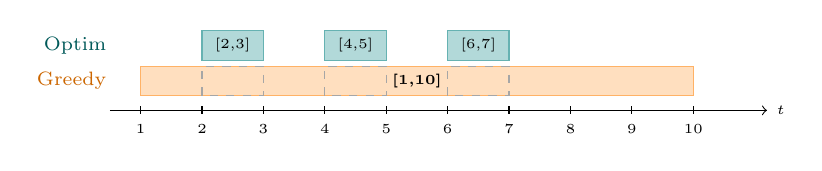
\begin{tikzpicture}[xscale=0.78, yscale=0.75]
    \draw[->] (0.5,-0.2) -- (11.2,-0.2) node[right,font=\tiny] {$t$};
    \foreach \xt in {1,2,...,10} {
      \draw (\xt,-0.13) -- (\xt,-0.27);
      \node[below,font=\tiny] at (\xt,-0.27) {\xt};
    }
    \node[left,font=\scriptsize,orange!80!black] at (0.6,0.3) {\alert{Greedy}};
    \fill[orange!25,draw=orange!60] (1,0.05) rectangle (10,0.55);
    \node[font=\tiny] at (5.5,0.3) {\textbf{[1,10]}};
    \draw[gray!70,dashed] (2,0.05) rectangle (3,0.55);
    \draw[gray!70,dashed] (4,0.05) rectangle (5,0.55);
    \draw[gray!70,dashed] (6,0.05) rectangle (7,0.55);
    \node[left,font=\scriptsize,teal!70!black] at (0.6,0.9) {Optim};
    \fill[teal!30,draw=teal!60] (2,0.65) rectangle (3,1.15);
    \node[font=\tiny] at (2.5,0.9) {[2,3]};
    \fill[teal!30,draw=teal!60] (4,0.65) rectangle (5,1.15);
    \node[font=\tiny] at (4.5,0.9) {[4,5]};
    \fill[teal!30,draw=teal!60] (6,0.65) rectangle (7,1.15);
    \node[font=\tiny] at (6.5,0.9) {[6,7]};
  \end{tikzpicture}
  \end{center}
\end{frame}

\begin{frame}{De ce nu sortăm după \textbf{durată}?}
  \textbf{Contraexemplu:} activități $[1,5],\ [4,6],\ [5,9]$
  \smallskip
  \begin{block}{Greedy după durată (crescătoare: $2,\ 4,\ 4$)}
    Ordine: $[4,6],\ [1,5],\ [5,9]$
    \begin{itemize}\itemsep2pt
      \item Alege $[4,6]$ \quad ($\mathit{last}=6$)
      \item $[1,5]$: $1 < 6$ \textemdash{} sare
      \item $[5,9]$: $5 < 6$ \textemdash{} sare
    \end{itemize}
    Rezultat: \alert{1 activitate}
  \end{block}
  \smallskip
  \begin{center}
  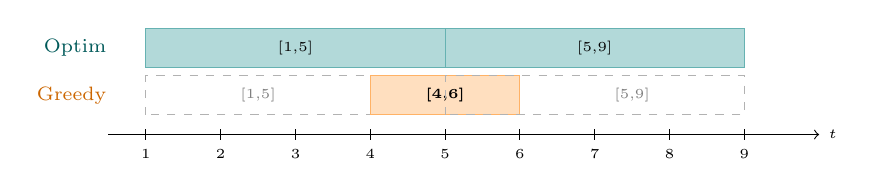
\begin{tikzpicture}[xscale=0.95]
    \draw[->] (0.5,-0.2) -- (10,-0.2) node[right,font=\tiny] {$t$};
    \foreach \xt in {1,2,...,9} {
      \draw (\xt,-0.13) -- (\xt,-0.27);
      \node[below,font=\tiny] at (\xt,-0.27) {\xt};
    }
    \node[left,font=\scriptsize,orange!80!black] at (0.6,0.3) {\alert{Greedy}};
    \draw[gray!60,dashed] (1,0.05) rectangle (5,0.55);
    \node[font=\tiny,gray] at (2.5,0.3) {[1,5]};
    \fill[orange!25,draw=orange!60] (4,0.05) rectangle (6,0.55);
    \node[font=\tiny] at (5,0.3) {\textbf{[4,6]}};
    \draw[gray!60,dashed] (5,0.05) rectangle (9,0.55);
    \node[font=\tiny,gray] at (7.5,0.3) {[5,9]};
    \node[left,font=\scriptsize,teal!70!black] at (0.6,0.9) {Optim};
    \fill[teal!30,draw=teal!60] (1,0.65) rectangle (5,1.15);
    \node[font=\tiny] at (3,0.9) {[1,5]};
    \fill[teal!30,draw=teal!60] (5,0.65) rectangle (9,1.15);
    \node[font=\tiny] at (7,0.9) {[5,9]};
  \end{tikzpicture}
  \end{center}
\end{frame}

\begin{frame}{Strategia corectă \textemdash{} sortare după \textbf{final}}
  \begin{block}{Criteriu}
    La fiecare pas, alege spectacolul care
    \textbf{se termină cel mai devreme} și nu se suprapune cu ultimul ales.
  \end{block}
  \smallskip
  \textbf{De ce funcționează?}
  \begin{itemize}\itemsep6pt
    \item Un spectacol care se termină mai devreme lasă
          \textbf{mai mult timp liber} pentru spectacolele viitoare
    \item Orice altă alegere (cu final mai târziu) lasă
          \textbf{cel mult la fel de mult timp liber} \textemdash{} niciodată mai mult
    \item Prin urmare, alegerea cu finalul cel mai mic este
          \textbf{întotdeauna la fel de bună sau mai bună}
  \end{itemize}
\end{frame}

\begin{frame}{Algoritmul}
  \begin{block}{Algoritm \textemdash{} Problema spectacolelor}
    \begin{enumerate}\itemsep6pt
      \item Sortează spectacolele după $f_i$ crescător
      \item Inițializează: $\mathit{cnt} \leftarrow 0$,\quad
            $\mathit{last} \leftarrow -\infty$
      \item \textbf{Pentru fiecare} spectacol (în ordine):\\
            dacă $s_i \geq \mathit{last}$:
            alege-l \quad ($\mathit{cnt}\texttt{++}$,\ $\mathit{last} \leftarrow f_i$)
    \end{enumerate}
  \end{block}
  \smallskip
  Parcurgerea este \textbf{liniară} \textemdash{} fiecare spectacol e inspectat o singură dată.
  Costul dominant este sortarea.
\end{frame}

\begin{frame}{Exemplu pas cu pas}
  \begin{center}
  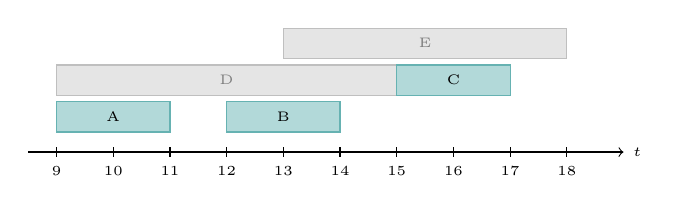
\begin{tikzpicture}[xscale=0.72, yscale=0.85]
    \draw[->] (0.5,-0.25) -- (11,-0.25) node[right,font=\tiny] {$t$};
    \foreach \xt in {9,10,...,18} {
      \pgfmathtruncatemacro{\xp}{\xt - 8}
      \draw (\xp,-0.18) -- (\xp,-0.32);
      \node[below,font=\tiny] at (\xp,-0.32) {\xt};
    }
    \fill[teal!30,draw=teal!60] (1,0.05) rectangle (3,0.5); \node[font=\tiny] at (2,0.28) {A};
    \fill[teal!30,draw=teal!60] (4,0.05) rectangle (6,0.5); \node[font=\tiny] at (5,0.28) {B};
    \fill[gray!20,draw=gray!50] (1,0.6) rectangle (7,1.05); \node[font=\tiny,gray] at (4,0.83) {D};
    \fill[teal!30,draw=teal!60] (7,0.6) rectangle (9,1.05); \node[font=\tiny] at (8,0.83) {C};
    \fill[gray!20,draw=gray!50] (5,1.15) rectangle (10,1.6); \node[font=\tiny,gray] at (7.5,1.38) {E};
  \end{tikzpicture}
  \end{center}
  \smallskip
  \begin{center}
  {\footnotesize
  \begin{tabular}{lccl}
    \toprule
    Spectacol & $s_i$ & $f_i$ & Decizie \\
    \midrule
    Film A & 9  & 11 & $9 \geq -\infty\ \checkmark$ \quad \textbf{ales} \quad ($\mathit{last}=11$) \\
    Film B & 12 & 14 & $12 \geq 11\ \checkmark$ \quad \textbf{ales} \quad ($\mathit{last}=14$) \\
    Film D & 9  & 15 & $9 < 14\ \times$ \quad \textcolor{gray}{sărit} \\
    Film C & 15 & 17 & $15 \geq 14\ \checkmark$ \quad \textbf{ales} \quad ($\mathit{last}=17$) \\
    Film E & 13 & 18 & $13 < 17\ \times$ \quad \textcolor{gray}{sărit} \\
    \bottomrule
  \end{tabular}}
  \end{center}
  \smallskip
  \textbf{Răspuns:} $\mathit{cnt} = 3$ \textemdash{} Film A, Film B, Film C.
\end{frame}

\begin{frame}[fragile]{Implementare}
\begin{lstlisting}
#include <bits/stdc++.h>
using namespace std;

struct Spectacol {
    int start, finish;
};

bool cmp(Spectacol a, Spectacol b) {
    return a.finish < b.finish;
}
\end{lstlisting}
  \begin{block}{Comparatorul \texttt{cmp}}
    Sortăm după \texttt{finish} (ora de final) crescător \textemdash{}
    exact criteriul greedy.
  \end{block}
\end{frame}

\begin{frame}[fragile]{Implementare}
\begin{lstlisting}
int main() {
    int n; cin >> n;
    vector<Spectacol> v(n);
    for (int i = 0; i < n; i++)
        cin >> v[i].start >> v[i].finish;

    sort(v.begin(), v.end(), cmp);

    int cnt = 0, last = -1;
    for (int i = 0; i < n; i++) {
        if (v[i].start >= last) {
            cnt++;
            last = v[i].finish;
        }
    }
    cout << cnt << "\n";
}
\end{lstlisting}
\end{frame}

\begin{frame}{Complexitate}
  \begin{center}
  \begin{tabular}{lll}
    \toprule
    Pas & Operație & Complexitate \\
    \midrule
    Citire     & $n$ spectacole    & $O(n)$ \\
    Sortare    & după ora de final & $O(n \log n)$ \\
    Parcurgere & o singură trecere & $O(n)$ \\
    \midrule
    \textbf{Total} & & $\mathbf{O(n \log n)}$ \\
    \bottomrule
  \end{tabular}
  \end{center}
  \smallskip
  \begin{block}{Spațiu și corectitudine}
    Spațiu: $O(n)$. Corectitudine: \textbf{exchange argument} \textemdash{}
    orice soluție optimă poate fi transformată în alegerea greedy
    fără a pierde activități.
  \end{block}
\end{frame}

% ============================================================
\section{Alte aplicații}

\begin{frame}{Selectarea celor mai profitabile $k$ elemente}
  \begin{block}{Problemă}
    Dintr-un tablou de $n$ valori, alege $k$ elemente astfel încât
    \textbf{suma lor să fie maximă}.
  \end{block}
  \smallskip
  \textbf{Strategie:} sortează descrescător $\rightarrow$ ia primele $k$ elemente.
  \smallskip
  \textbf{Exemplu:} $a = [3, 7, 1, 9, 4]$, $k = 3$
  \begin{itemize}
    \item Sortat: $[9, 7, 4, 3, 1]$
    \item Suma: $9 + 7 + 4 = 20$ \quad \textcolor{gray}{(optim)}
  \end{itemize}
  \smallskip
  \textbf{Corectitudine:} înlocuind orice element din top $k$
  cu unul mai mic, suma ar \textbf{scădea}.
  \smallskip
  \textbf{Complexitate:} $O(n \log n)$
\end{frame}

\begin{frame}{Acoperire cu intervale \textemdash{} Enunț}
  \begin{block}{Problemă}
    Se dau $m$ intervale $[l_i, r_i]$.
    Acoperă segmentul $[0, L]$ complet
    folosind \textbf{cât mai puține intervale}.
  \end{block}
  \smallskip
  \begin{block}{Strategie greedy}
    Fie $\mathit{pos}$ = capătul drept acoperit până acum (inițial $0$).
    La fiecare pas:
    \begin{enumerate}
      \item Consideră toate intervalele cu $l_i \leq \mathit{pos}$
      \item Alege cel cu $r_i$ \textbf{maxim}
      \item Actualizează $\mathit{pos} \leftarrow r_i$
    \end{enumerate}
    Repetă până când $\mathit{pos} \geq L$.
  \end{block}
\end{frame}

\begin{frame}{Acoperire cu intervale \textemdash{} Exemplu}
  $L = 10$, intervale:
  $[0,4],\ [1,7],\ [2,5],\ [5,10],\ [6,12]$
  \smallskip
  \begin{center}
  \begin{tabular}{ccll}
    \toprule
    Pas & $\mathit{pos}$ & Eligibile ($l \leq \mathit{pos}$) & Ales \\
    \midrule
    1 & $0$ & $[0,4]$ & $[0,4]$ $\rightarrow$ $\mathit{pos}=4$ \\[3pt]
    2 & $4$ & $[1,7],\ [2,5]$ & $[1,7]$ (max $r$) $\rightarrow$ $\mathit{pos}=7$ \\[3pt]
    3 & $7$ & $[5,10],\ [6,12]$ & $[6,12]$ (max $r$) $\rightarrow$ $\mathit{pos}=12$ \\
    \bottomrule
  \end{tabular}
  \end{center}
  \smallskip
  $\mathit{pos} = 12 \geq 10 = L$ \textemdash{} acoperit complet.
  \smallskip
  \textbf{Răspuns:} $3$ intervale: $[0,4],\ [1,7],\ [6,12]$.
\end{frame}

\begin{frame}{Limitele abordării Greedy}
  \begin{alertblock}{Greedy nu este mereu corect!}
    Trebuie să argumentăm că alegerea locală optimă
    conduce la soluția globală optimă.
  \end{alertblock}
  \smallskip
  \textbf{Cum verificăm corectitudinea?}
  \begin{enumerate}\itemsep8pt
    \item \textbf{Exchange argument} \textemdash{} presupui că există o soluție mai bună
          și arăți că o poți transforma în alegerea greedy fără a pierde calitate
    \item \textbf{Testare empirică} \textemdash{} compară cu brute force pe cazuri
          mici ($n \leq 15$)
    \item \textbf{\textit{Proof by AC}} \textemdash{} trimiți direct la judge
          și verifici (metodă comună la concursuri)
  \end{enumerate}
\end{frame}

% ============================================================
\section{Recapitulare}

\begin{frame}{Recapitulare}
  \begin{center}
  \begin{tabular}{lll}
    \toprule
    Problemă & Criteriu greedy & Complexitate \\
    \midrule
    Spectacole          & Sortare după final       & $O(n \log n)$ \\
    $k$ elemente maxime & Sortare descrescătoare   & $O(n \log n)$ \\
    Monede standard     & Cea mai mare $\leq$ rest & $O(n)$ \\
    Acoperire intervale & Extindere maximă         & $O(n \log n)$ \\
    \bottomrule
  \end{tabular}
  \end{center}
  \smallskip
  \textbf{Pași tipici:}
  \begin{enumerate}
    \item Identifică \textbf{criteriul de ordonare}
    \item Sortează $+$ parcurge \textbf{liniar}
    \item Verifică \textbf{corectitudinea} (exchange argument / empiric)
  \end{enumerate}
\end{frame}

\begin{frame}{Probleme de antrenament}
  \begin{enumerate}\itemsep6pt
    \item \href{https://cses.fi/problemset/task/1094}{\textbf{Increasing Array}}
          \textcolor{gray}{(CSES \#1094)}
    \item \href{https://atcoder.jp/contests/abc088/tasks/abc088_b}{\textbf{Card Game for Two}}
          \textcolor{gray}{(AtCoder ABC088 B)}
    \item \href{https://cses.fi/problemset/task/1084}{\textbf{Apartments}}
          \textcolor{gray}{(CSES \#1084)}
    \item \href{https://cses.fi/problemset/task/1090}{\textbf{Ferris Wheel}}
          \textcolor{gray}{(CSES \#1090)}
    \item \href{https://cses.fi/problemset/task/1629}{\textbf{Movie Festival}}
          \textcolor{gray}{(CSES \#1629)}
    \item \href{https://cses.fi/problemset/task/1630}{\textbf{Tasks and Deadlines}}
          \textcolor{gray}{(CSES \#1630)}
  \end{enumerate}
\end{frame}

\begin{frame}{Resurse}
  \begin{enumerate}\itemsep10pt
    \item \href{https://www.pbinfo.ro/articole/16619/metoda-greedy}{\textbf{pbinfo}}
          \textemdash{} Metoda Greedy (în română)
    \item \href{https://usaco.guide/bronze/intro-greedy}{\textbf{USACO Guide}}
          \textemdash{} Introduction to Greedy Algorithms (Bronze)
    \item \href{https://usaco.guide/silver/greedy-sorting}{\textbf{USACO Guide}}
          \textemdash{} Greedy Algorithms with Sorting (Silver)
    \item \href{https://cses.fi/book/book.pdf}{\textbf{CPH}}
          \textemdash{} cap.\@ 6 \textemdash{} Greedy Algorithms
  \end{enumerate}
\end{frame}

\end{document}
